In this case, the SOC of the battery is set at 94\% as the initial SOC and the supercapacitor’s initial voltage is kept 535V with SOC of 97.02\%.

In this case, the same steps of the case 1 and case 2 are performed. From Fig. \ref{ch5_f117}, the simulation results up to $t$ = 2s  are the same as shown earlier in case 1, whereas at $t$ = 0.3s, $t$ = 0.6s and $t$ = 1s to $t$ = 2s,  34MW, 6MW and 4MW pulsed load are connected to MVDC system, respectively. From Fig. \ref{ch5_f117}, the FL controller based ESM system provides negative $P_{stor-ref}$ for discharging of the battery and supercapacitor and to supply power to the MVDC system. At $t$ = 2.5s, 4MW load is rejected and the FL controller based ESM system is expected to provide the positive $P_{stor-ref}$ for charging. But from Fig. \ref{ch5_f117}, the charging reference power ($P_{stor-ref}$) generated by the FL controller based ESM system is zero. This is because the reference power generation by the FL controller based EMS system depends on the SOC of the battery and supercapacitor with other two input variables. Due to the high SOC (nearly 94\% and 97.02\%) of the battery and supercapacitor, Fig. \ref{ch5_f117} shows that the FL controller based ESM system provides zero reference power for charging to avoid overcharging. From the Figure \ref{ch5_f117}, it is clear that the Off-line and CHIL results are same. 
  
%gfhgfhfgjhg
%fghgfhg
\begin{figure}[ht!]
\begin{subfigure}{1\columnwidth}
\begin{center}
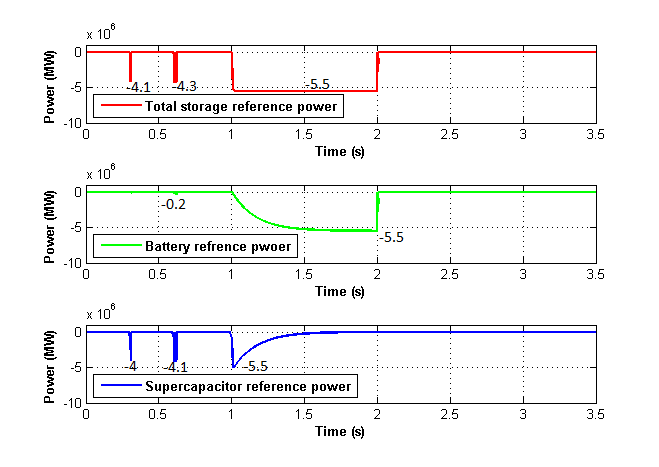
\includegraphics[height=3in, width=3.5in]{f117b}
\end{center}
\caption{Off-line simulation results.}
\label{ch5_f117b}
\end{subfigure}
\begin{subfigure}{1\columnwidth}
\begin{center}
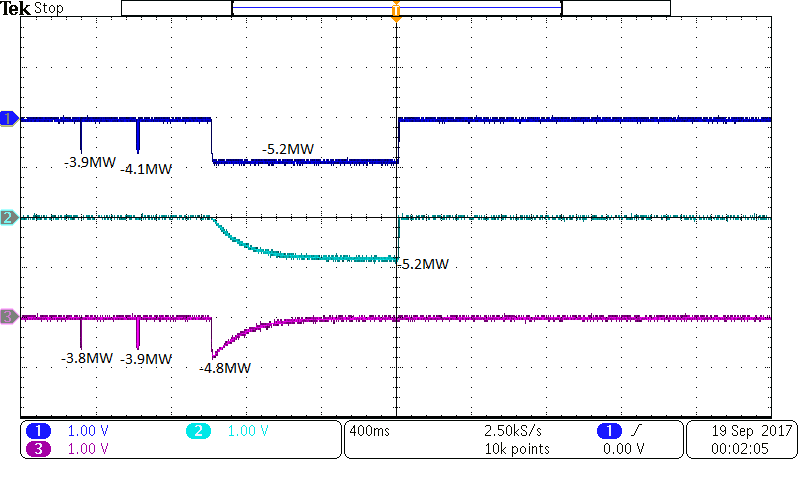
\includegraphics[height=2in, width=3.5in]{f117}
\end{center}
\caption{CHIL results-oscilloscope plots: Ch1: total storage reference power, Ch2: battery reference power, Ch3: supercapacitor reference  power (Ch1, Ch2, Ch3 = 5MW/div).}
\label{ch5_f117a}
\end{subfigure}
\caption{Reference power produced by FL controller and LPF based ESM system (case 3).}
\label{ch5_f117}
\end{figure}



